\subsection{Netzkommunikation}
Die Kommunikation in einem Netzwerk findet über s.g. Netzprotokolle statt. So wird gewährleistet, dass der Sender und der Empfänger die selbe "Sprache" sprechen. Wird z.B. eine Web Seite in einem Browser aufgerufen, wir meist das HTTP-Protokoll verwendet. Dieses wird über weitere Protokolle in ein Paket gepackt, und an den gewünschten Web Server gesendet. Dieser entpackt das Paket in umgekehrter Reihenfolge wie der Sender, und gelangt so letztendlich zur ursprünglichen Nachricht. Für die Reihenfolge der anzuwendenden Protokolle gibt es zwei Grundlegende Referenzmodelle:\\
\\
\noindent\textbf{OSI-Referenzmodell}\\
\noindent Das  OSI-Schichtenmodell beschreibt die Struktur der gesamten Kommunikation zweier Kommunikationsteilnehmer. Es besteht aus sieben Schichten, die aus jeweils mehreren Protokollen bestehen, die für unterschiedliche Aufgabenstellungen zuständig sind:\\
\begin{itemize}
\item Anwendungsschicht: Diese Schicht sorgt für eine Umsetzung der Anforderungen der Anwendung
\item Darstellungsschicht: Diese Schicht sorgt dafür das die Nachricht in eine für die Anwendung verwertbare Sprache zur Verfügung gestellt wird
\item Kommunikationsschicht: Diese Schicht kümmert sich um den Aufbau und Überwachung von Verbindungen
\item Transportschicht: Diese Schicht sorgt für eine transparente Ende-zu-Ende Verbindung mit einem Kommunikationspartner
\item Vermittlungsschicht: Die Vermittlungsschicht kümmert sich um die Vermittlung der oberen Schichten. Zu ihren Aufgaben gehören unter anderem das Routing und die Adressierung.
\item Sicherungsschicht: Diese Schicht bietet Funktionen wie Fehlerkorrekturen und Flusssteuerung an
\item Bitübertragungsschicht: Die unterste Schicht behandelt die physikalische Verbindung zweier Punkte und ist für die Bitstream-Übertragung zuständig 
\end{itemize}

\noindent Die Kommunikation über diese Schichten findet über Paketen statt, die z.B. in der Anwendungsschicht erstellt, und danach in die darauf folgenden sechs Schichten gekapselt verpackt werden. Beim Empfänger werden die Schichten zur Anwenderschicht wieder entfernt bis die eigentliche Nachricht interpretierbar wird. In Abb. \ref{osi} wird ein Beispielkommunikation über das Internet dargestellt.\\
\begin{figure}[h]
    \centering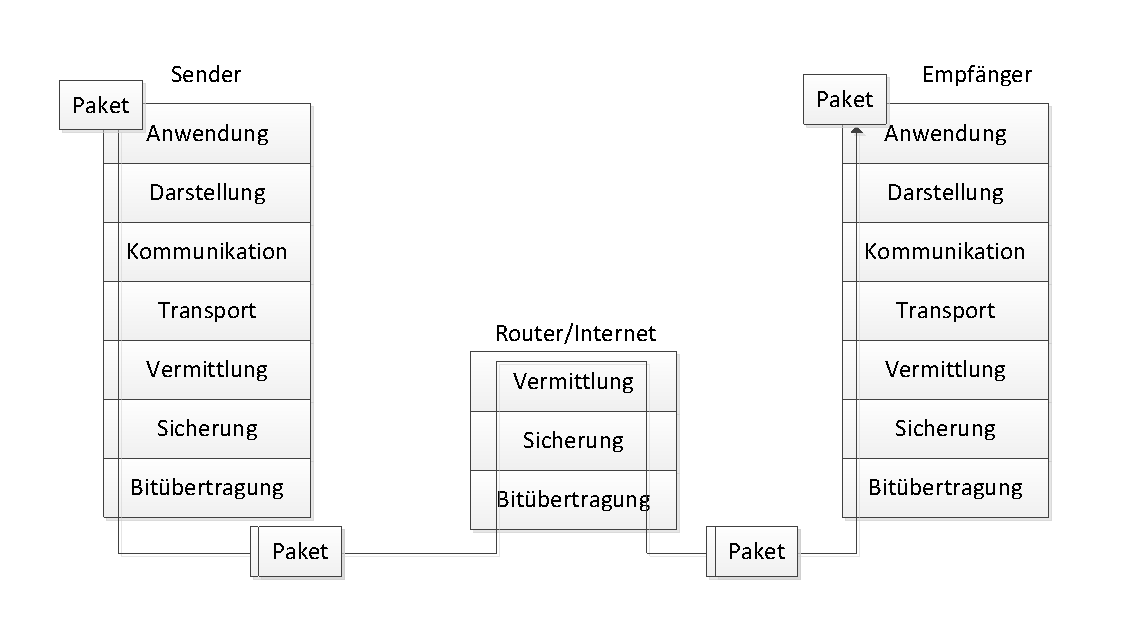
\includegraphics[scale=0.7]{Bilder/OSI.pdf}
  \caption{Kommunikation über das OSI-Schichtenmodell}
  \label{osi}
\end{figure}

\noindent Das OSI-Schichtenmodell wir häufig als Grundlage für den Entwurf neuer Netzwerkprotokolle verwendet. In der Realität finden Kommunikation meist über weniger Schichten statt, wie z.B. das TCP/IP-Referenzmodell.\\

\noindent\textbf{TCP/IP-Referenzmodell}\\
\noindent Das TCP/IP-Referenzmodell basiert auf dem OSI-Modell, fasst jedoch die Aufgaben einiger Schichten zusammen. So wird satt der Bitübertragungs- und Sicherungsschicht eine allgemeine Netzzugangsschicht, und aus Kommunikations-, Darstellungs-, und Anwendungsschicht eine allgemeine Anwendungsschicht. Die Vermittlungs-, und Transportschicht werden beibehalten. \\
